%-------------------------------------------------------------------------------
%	PAQUETES Y OTRAS CONFIGURACIONES
%-------------------------------------------------------------------------------

%-------------------------------------------------------------------------------
%	PAQUETES Y OTRAS CONFIGURACIONES
%-------------------------------------------------------------------------------
\documentclass{tufte-handout}
%\documentclass[paper=letter, fontsize=11pt]{scrartcl} % Tamaño de papel y letra para el documento
\usepackage{geometry}
\geometry{left=1.2cm, right=6.2cm, top=2.5cm, bottom=2.5cm}
\usepackage{color}
\usepackage[utf8]{inputenc} % Los caracteres acentuados se pueden escribir normalmente en el código
\usepackage[T1]{fontenc} % Configuración de fuente de salida
\usepackage{cmbright}
\usepackage[sfdefault]{noto}
\usepackage[T1]{fontenc}
\normalfont
\usepackage{graphicx} % Paquetes para incluir imágenes
\usepackage{multicol}
\usepackage{circuitikz}
\usepackage{tikz}
\usetikzlibrary{arrows}

\usepackage{sectsty} % Paquete para configuración de secciones
\allsectionsfont{\centering \normalfont \scshape} % Los títulos de las secciones son centrados, con la misma fuente y pequeñas mayúsculas

\usepackage{todonotes}
\usepackage{microtype}
\renewcommand{\figurename}{Figura}

\usepackage{listings}
\renewcommand{\lstlistingname}{Código}
\lstdefinestyle{mystyle}{
    basicstyle=\footnotesize,
    breakatwhitespace=false,
    breaklines=true,
    captionpos=b,
    keepspaces=true,
    numbers=left,
    numbersep=5pt,
    showspaces=false,
    showstringspaces=false,
    showtabs=false,
    tabsize=2
}
\lstset{style=mystyle}

% \usepackage{fancyhdr} % Paquete para personalizar pies y cabeceras de página
% \pagestyle{fancyplain} % Todas las páginas con las mismas cabeceras y pies de página
% \fancyhead{} % Sin cabecera
% \fancyfoot[L]{} % Vacío en la izquierda del pie de página
% \fancyfoot[C]{} % Vacío en el centro del pie de página
% \fancyfoot[R]{\thepage} % Número de página en el pie de pagina
% \renewcommand{\headrulewidth}{0pt} % Sin lineas en la cabecera
% \renewcommand{\footrulewidth}{0pt} % Sin lineas en el pie de página
% \setlength{\headheight}{13.6pt} % Altura de cabecera
%
% \numberwithin{equation}{section} % Numera ecuaciones en cada sección
% \numberwithin{figure}{section} % Numera figuras en cada sección
% \numberwithin{table}{section} % Numera tablas en cada sección
%
% \setlength\parindent{0pt} % Quita la indentación de los párrafos

\newcommand{\horrule}[1]{\rule{\linewidth}{#1}} % Comando personalizado para hacer linea horizontal


%-------------------------------------------------------------------------------
%	TITULO
%-------------------------------------------------------------------------------

\title{Práctica 0 - Ejemplo de Reporte de Práctica\\Interfaces y periféricos para robots}
\author{Roberto Cadena Vega} % Nombre del profesor
\date{}

%-------------------------------------------------------------------------------
%	EMPIEZA EL DOCUMENTO
%-------------------------------------------------------------------------------

\begin{document}

\maketitle % Imprime el título

%-------------------------------------------------------------------------------
%	OBJETIVOS
%-------------------------------------------------------------------------------

\section{Introducción}

	Familiarizarse con el formato general para la entrega de reporte de prácticas. \footnote{Con formato me refiero a la estructura general del documento, no a las especficaciones esteticas de este. Nota que el espacio al margen es utilizado raramente, por lo que es un buen lugar para hacer anotaciones.}

%-------------------------------------------------------------------------------
%	CONOCIMIENTOS PREVIOS
%-------------------------------------------------------------------------------

\subsection{Conocimientos Previos}

%-------------------------------------------------------------------------------

	%\subsection{Práctica}

		Dentro de las prácticas que se desarrollen en el laboratorio, tendrás que realizar circuitos eléctricos y realizar mediciones con el equipo del laboratorio, por lo que es muy importante que sepas como tienes que reportar tus resultados. \\

		Hay varios elementos importantes dentro de un reporte de práctica, pero siempre tienes que tener en cuenta que un reporte de práctica te tiene que servir para replicar tus resultados posteriormente (para ti o para quien sea que los tenga que revisar). \\

		Lo primero de lo que podemos hablar es de los conocimientos previos a la práctica, y estos se refieren al marco teórico que encuadra la práctica. \\

		Por ejemplo, para analizar un circuito eléctrico necesitamos hablar de la ley de Ohm, por lo que podemos mencionarla\footnote{Nota como la formula se muestra correctamente a pesar de tener simbolos latinos y griegos, subscritos y superscritos.}:

		\begin{equation}
			V_T = I_T \cdot R_T = 0.36 A \cdot 330 \Omega = 120 V
		\end{equation}

		y hablar brevemente de que significa cada termino y la relación entre ellos. \\

		Antes de poder entrar al laboratorio para realizar tu práctica, se te pedirá que entregues un cuestionario resuelto, para lo cual tendrás que haber leido la especificación de práctica proveida por el profesor, e investigado cualquier otra cosa necesaria para poder contestarlo correctamente. \\

%-------------------------------------------------------------------------------
%	EQUIPO
%-------------------------------------------------------------------------------

\subsection{Equipo}

	El equipo de laboratorio se refiere a todo aquel material o herramienta necesaria para realizar el circuito eléctrico en el laboratorio, pero que no esta directamente involucrado en el circuito eléctrico. Ejemplos de equipo, son los siguientes:

	\begin{itemize}
		\item Fuente de Alimentación
		\item Osciloscopio
		\item Generador de Funciones
		\item Multimetro
		\item Cables de alimentación
		\item Cables banana - caimán
		\item Pinzas
	\end{itemize}

%-------------------------------------------------------------------------------
%	MATERIALES
%-------------------------------------------------------------------------------

\subsection{Materiales}

	Los materiales son todos los elementos que si estan involucrados en el circuito eléctrico:

	\begin{itemize}
		\item Protoboard
		\item LED (no importa el color, aunque los difusos son mas fáciles de ver en las condiciones de iluminación del laboratorio)
		\item Resistencias
		\begin{itemize}
			\item $220 \Omega$
			\item $330 \Omega$
			\item $1 k\Omega$
		\end{itemize}
		\item Cables
	\end{itemize}

%-------------------------------------------------------------------------------
%	DESARROLLO
%-------------------------------------------------------------------------------

\section{Desarrollo}

    El desarrollo es una descripción con tus propias palabras de el procedimiento de construcción del circuito y toma de las mediciones requeridas, asi como de cualquier calculo necesario. Este puede tener diagramas esquematicos o representativos de tus cricuitos, pero \textbf{no} debe de tener fotografías; se considerarán correctos diagramas realizados con computadora, o a mano y digitalizados por medio de scanner.\footnote{Si se sorprende al alumno utilizando recursos de otro autor, sin dar el correspondiente credito se le serán deducidos puntos.} Un ejemplo de diagrama esquemático lo podemos ver en la figura \ref{dia:elecir}. \\

    \begin{marginfigure}%[h]
    	\begin{center}
    		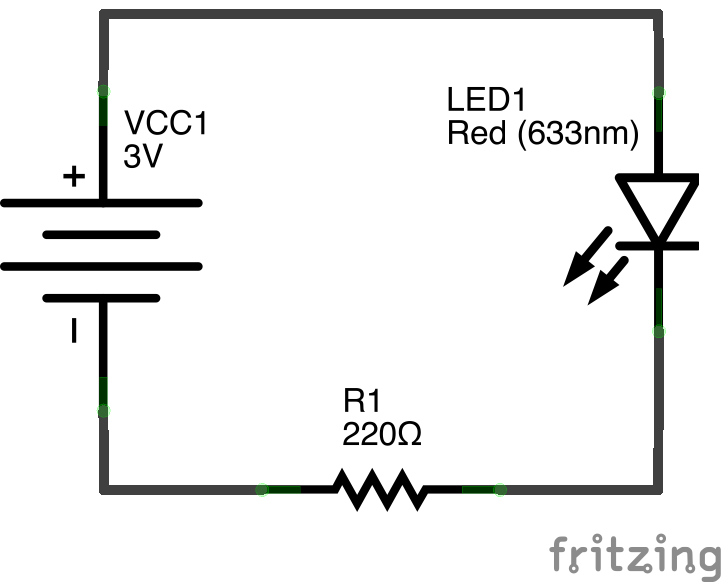
\includegraphics[width=\textwidth]{images/LED-bateria-diagrama.png}
    		\caption{Diagrama eléctrico del circuito a ensamblar.}
    		\label{dia:elecir}
    	\end{center}
    \end{marginfigure}

    Un diagrama representativo de un circuito se puede ver en la figura \ref{dia:cir}. \\

    \begin{marginfigure}%[h]
    	\begin{center}
    		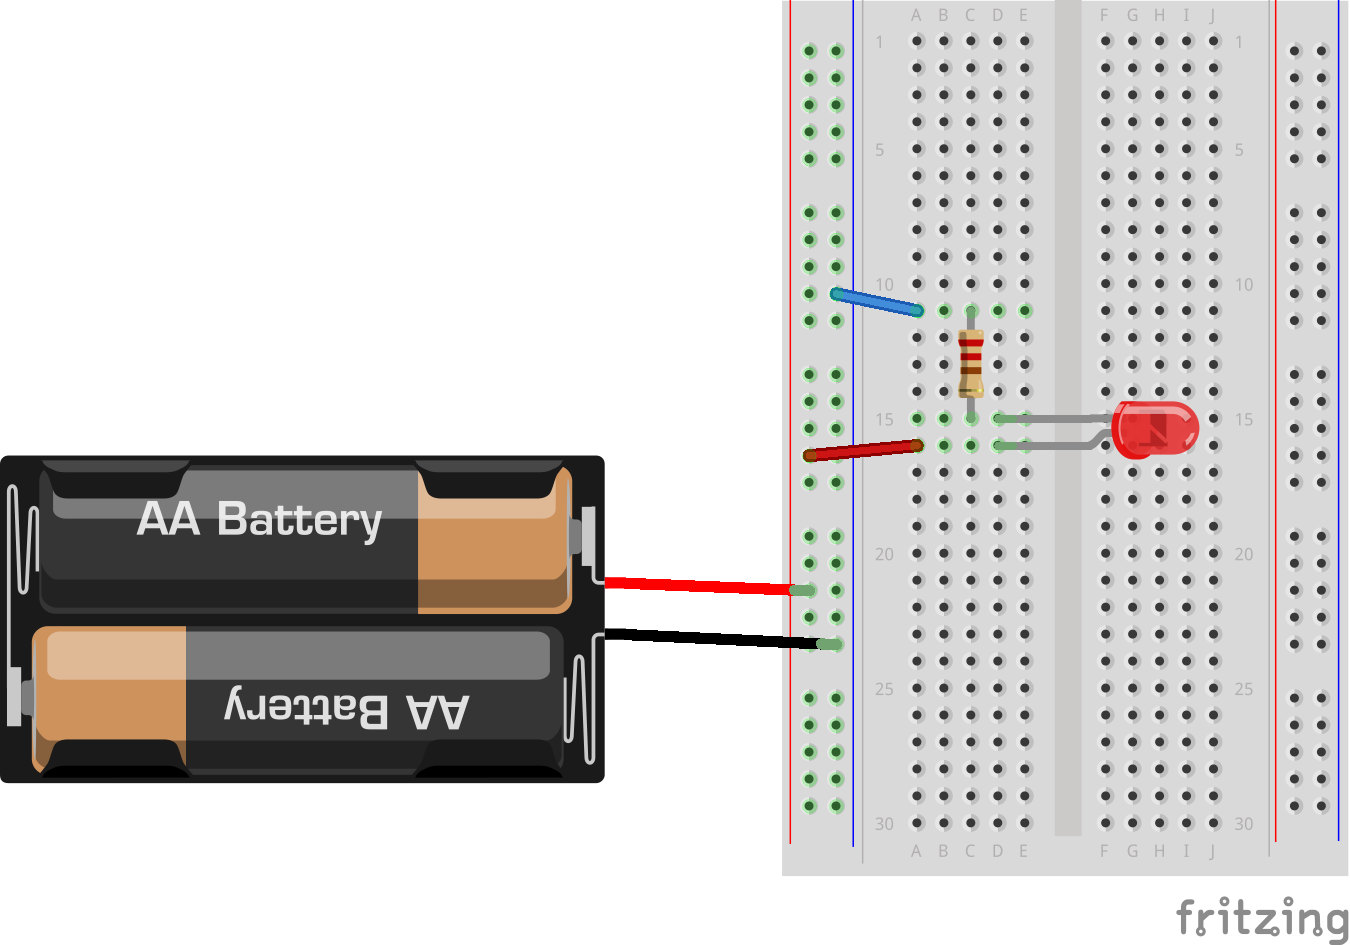
\includegraphics[width=\textwidth]{images/LED-bateria.png}
    		\caption{Diagrama del circuito a ensamblar.}
    		\label{dia:cir}
    	\end{center}
    \end{marginfigure}

    Durante el desarrollo de la práctica se te pedirá que realices diversas mediciones, las cuales tendrás que anotar en la hoja indicada para ello. En cada práctica esta hoja es diferente, y te dará una buena idea de cuales son los elementos indispensables\footnote{Indispensables significa necesarios, mas no suficientes.} en tu reporte de práctica. \\

%-------------------------------------------------------------------------------
%	CONCLUSIONES
%-------------------------------------------------------------------------------

\section{Conclusiones}
	Las conclusiones de una práctica deben de ser tanto vivenciales, como orientadas al objetivo marcado al principio de la práctica. Pueden ser tanto positívos, como negatívos; dependiendo de los resultados obtenidos en el laboratorio. \\

	Recuerda que la calificación de la práctica depende tanto del trabajo que realices en el laboratorio, como de lo preciso de tu reporte. \\

	La longitud máxima del reporte aceptable es de 5 páginas. \\

	La entrega de los reportes se hará en formato PDF (sin excepciones) por medio de la plataforma Blackboard. \\

	Recuerda que para que tu práctica sea considerada tambien debes de entregar tu hoja de anotaciones revisada por el profesor.

%-------------------------------------------------------------------------------
%	FIN DEL DOCUMENTO
%-------------------------------------------------------------------------------

\end{document}
